11. \begin{figure}[ht!]
\center{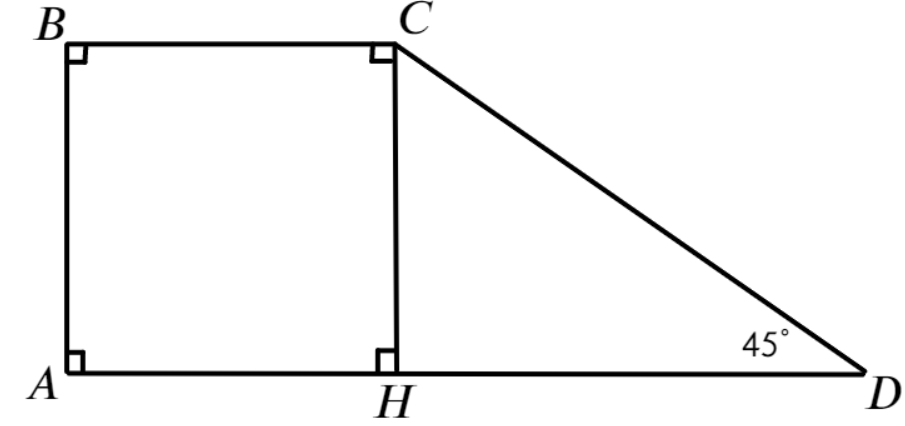
\includegraphics[scale=0.35]{g8-11.png}}
\end{figure}\\
Опустим из точки $C$ высоту $CH.$ Так как $AB=BC,$ четырёхугольник $ABCH$ является квадратом, поэтому $CH=AH=AB=6$ см. Найдём $\angle D=180^\circ-\angle C=180^\circ-135^\circ=45^\circ,$ поэтому $\angle HCD=180^\circ-90^\circ-45^\circ=45^\circ$ и треугольник $CHD$ является равнобедренным, $CH=HD.$ Тогда $AD=AH+HD=6+6=12$см и $S_{ABCD}=\cfrac{1}{2}\cdot6\cdot(6+12)=54\text{см}^2.$\\
